\section{Introduction}

Parking lots present a difficult search problem. Lacking enough visibility to
determine where spots are available, drivers may search fruitlessly through
lot after lot, wasting time and energy while generating harmful vehicle
emissions. And while some high-demand lots in urban areas and at airports
have been instrumented to monitor availability, the high cost of the
equipment required has prevented this approach from being widely-deployed at
many lots where drivers find themselves searching for spots, including at
university campuses and suburban shopping malls. Our own campus featuring 40
lots with over 80 entrances would cost at least \$\num{28000} to monitor even
with the least expensive research prototype~\cite{propst2012embedded} and an
order-of-magnitude more with available commercial
solutions~\cite{car-detect}. Instead of relying on additional infrastructure,
we believe a free solution is already in our pockets.

\textit{PocketParker} is a system that predicts parking lot availability
using smartphones. Unlike previous approaches, our approach requires no
additional infrastructure, no vehicle modifications, and no user interaction,
only the installation of a smartphone app. PocketParker runs unattended in
the background and uses activity transitions to detect parking lot arrivals
and departures. These are forwarded to a central server that incorporates
them into per-lot availability models. This allows PocketParker to order lots
accurately by the probability that they contain an available spot. We
consider PocketParker an example of a subset of crowdsourcing that does not
require any user input which we call \textit{pocketsourcing}.

Predicting parking availability requires accurately detecting parking events
as well as determining the effect of \textit{hidden drivers}---drivers not
using PocketParker---on lot availability. We address the first challenge with
a simple, effective, and energy-efficient event detector which uses
accelerometer data to detect vehicle arrivals and departures. The second goal
we achieve with an availability estimator that maintains a probability model
for each lot by incorporating events generated by PocketParker clients.
Parking events are used both to model arrival and departure rates and to
estimate the number of hidden drivers. One key insight is that even without
monitoring all drivers there are moments when PocketParker is certain that a
parking spot is available in a particular lot and can use this information to
assist users.

Our paper makes the following contributions. After motivating our approach
through an examination of related work, we present the design of PocketParker
in detail, describing in separate sections how PocketParker detects parking
events and maintains per-lot availability models. We then perform a thorough
evaluation of each component of PocketParker and the performance of the
system as a whole. We test our parking event detector in a controlled
environment with eight volunteers participating in ten parking scenarios. We
test our parking availability estimator with a simulator providing the
ability to experiment with a variety of parking lot configurations and
arrival and departure rates.

Finally, we test the end-to-end effectiveness of PocketParker through a field
trial involving 105~smartphones users that generated \num{10827} parking
events over 45~days. To obtain ground truth, we deployed four cameras to
monitor two parking lots over two weeks and hand-coded four days' worth of
images to measure their true availability. Our results demonstrate that
PocketParker can accurately and efficiently detect parking events and use
them to make accurate availability predictions. During the field trial it was
able to correctly predict lot availability 94\% of the time.

We evaluate the system using a number of methods.  We test our parking event
detector in a controlled environment with eight volunteers participating in
ten parking scenarios. We test our parking availability estimator with a
simulator that gives us the flexibility to experiment with a variety of
parameters and parking lot types.  We test the overall effectiveness of
PocketParker in a field trial involving 105 smartphones users over forty five
days. To obtain ground truth, we deploy four cameras that monitor two parking
lots over two weeks. We inspect and hand-code four days' worth of images of
these lots to measure their true availability.

Structurally, our paper describes each system component in detail. We start
our discussion by presenting related works in parking monitoring and their
distinctions from PocketParker.  The next two sections describe two major
components of PocketParker: our parking event detector and availability model.
The third part, our evaluation, is based both on simulations, controlled
experiments, and a prototype deployment involving 105 users.  Finally, we
discuss limitations and future work.

Installation costs for parking systems can be significant: \$18 million for
monitoring and collection equipment for \num{7000} street spots in the SFPark
system~\cite{sfpark}. For lot parking, inexpensive systems have been proposed
that simply track lot counts~\cite{propst2012embedded}. In practice, a
permanant infrastructure for such an approach would involve permanant
mounting and communication for each sensor. For comparison, the real cost of
an installed vehicle detector including wireless transponder is about
\$\num{9700}~\cite{car-detect}. Communication link costs alone can run
\$\num{4600}~\cite{mstp-park}. Apart from instrumentation, the data collected
needs to be relayed to drivers. One programmable sign to advertise lot
availability can cost \$\num{49000}~\cite{mstp-park}. Scaling these figures
compounds the cost: our own campus setting involves over 40 major lots with
over 80 separate entrances.

The advent of mobile smartphones has invited manifold new approaches to the
problem of communicating parking availability.  Online sites such as the
Google App Play Store teem with proposed solutions.  Presently, however, these
apps either do not provide real-time parking lot availability or they simply
display publicly-available information. Several research projects have
attempted to address these limitations~\cite{4212497, Chen:2012:COS,
Delot:2009:CRP, 5062057, Mathur:2010:PDS} but include requirements rendering
them impractical to mass rollout.  They either require additional
infrastructure~\cite{5062057}, on-vehicle equipment~\cite{Mathur:2010:PDS}
or networking~\cite{Delot:2009:CRP, Mathur:2010:PDS}, or onerous manual user
input~\cite{Chen:2012:COS}. In contrast, we suggest, the solution is already
in peoples' pockets.


\begin{comment}
\begin{figure}
\centering
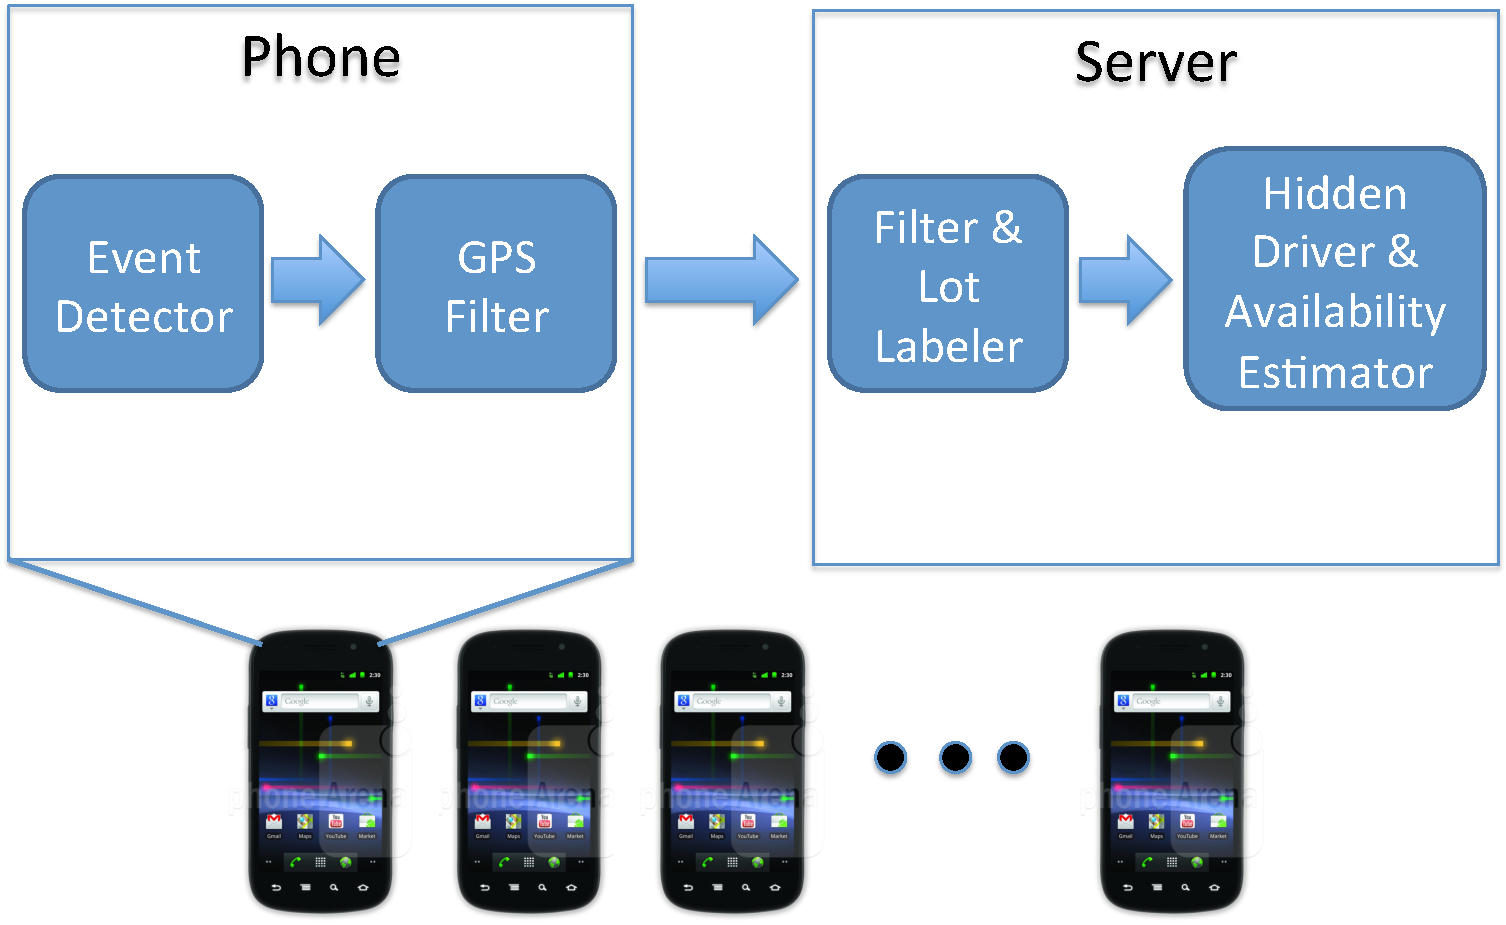
\includegraphics[height=1.5in]{./figures/blockdiagram.pdf}

\caption{\textbf{The PocketParker architecture.} Events generated by an
activity detector running quietly on each smartphone are processed by a
central server and used to estimate parking lot availability.}

\label{fig-arch}
\vspace*{-0.2in}
\end{figure}
\end{comment}
